% Não é preciso declarar nenhum cabeçalho

\section{Transporte}
\subsection{Voltar para casa}

Para os calouros de fora de Campinas, além de escolher a nova morada é
importante reunir informações sobre como realizar o trajeto entre sua cidade e
Campinas.

A forma usual é ir de ônibus, mas tenha em mente que a rodoviária é longe e os
trajetos de ônibus até lá são demorados. O endereço da rodoviária é: Rua Pereira
Lima, s/n. Há duas linhas que passam por lá: o 332 (Para no Hospital das Clínicas)
para dentro da rodoviária, mas demora mais pra chegar que o 331, que sai do
terminal e para do lado de fora da rodoviária. Em horários de pico, o trajeto
pode demorar quase uma hora, então cuidado para não perder o horário do ônibus
para sua cidade. Também não se esqueça de portar algum cartão para andar nos
ônibus de Campinas, seja o Bilhete Único ou um dos dois cartões avulsos (Bilhete
1 Viagem e Bilhete 2 Viagens). Caso contrário, não será possível embarcar em um
ônibus.

Os que vêm de mais longe certamente farão uso do aeroporto de Viracopos, cujo
telefone é 3725-5000. Para chegar ao aeroporto existe a linha 193 que sai da
rodoviária e vai para o aeroporto, e também faz o trajeto de volta. Porém, ir
com ônibus circular pode ser um transtorno quando estiver com muita bagagem. Uma
outra alternativa é a Lirabus que também faz o traslado da rodoviária para o
aeroporto. A passagem da Lirabus custa R\$9,00 (R\$9,80 se sair da Rodoviária,
pois paga taxa de embarque) e os horários podem ser conferidos no site
\url{www.lirabus.com.br/}.

Para quem for usar os aeroportos da Grande São Paulo (Congonhas e Guarulhos),
existem os serviços de traslado, também oferecidos pela Lirabus. A tarifa para
Guarulhos sai R\$28,30 (R\$33,70 com taxa de embarque da Rodoviária), e para
Congonhas sai R\$24,45 (R\$29,90 com taxa de embarque da Rodoviária).

Para não pagar a taxa de embarque nos traslados da Lirabus, basta embarcar na
Sala VIP da Lirabus, localizada na Avenida Francisco Glicério, 435, em frente ao
Largo do Pará.

\subsubsection{Caronas}

Uma forma barata e divertida de viajar, além de minimizar o tempo e dinheiro
gastos na viagem, é juntando alguns estudantes no mesmo carro e dividir as
despesas.
\begin{figure}[h!]  \centering
    \includegraphics[width=.45\textwidth]{img/barao/unicaronas.jpg}
\end{figure}

O site UniCaronas (\url{unicaronas.com.br}) foi desenvolvido por dois
engenheiros de computação da Unicamp, com o intuito de facilitar o deslocamento
dos alunos entre cidades. Criado em 2007 como Caronas Unicamp e disponível
apenas para alunos da Unicamp, O site chegou a possuir mais de 20 mil usuários e
mediar caronas entre alunos de diversas universidades para várias cidades de
vários estados. Em 2014, o site se uniu ao Tripda (\url{tripda.com.br}),
aumentando imensamente a quantidade de destinos, mas mantendo as funcionalidades
básicas. No entanto, o site serve apenas para colocar os motoristas e caronistas
em contato, não assumindo responsabilidades sobre nenhuma das partes.

Recentemente foi criado o Mural de Caronas\\(\url{muraldecaronas.org}), que
igualmente ao UniCaronas exige um email institucional para realização do
cadastro no site. Entretanto, por enquanto só há opção de carona entre Barão
Geraldo e São Paulo. Além disso, há varios grupos de carona no Facebook, vale a
pena checá-los.

\subsection{Carro}

Para aqueles que tenham seu próprio veículo, é bom saber que a Unicamp tem
poucas vagas próximas aos locais de aulas. E o número de fiscais de trânsito tem
aumentado muito dentro do Campus.

\subsubsection{Autoescolas}

Se você ainda não tem CNH e pretende obtê-la em Campinas, existem três opções de
autoescola em Barão Geraldo:

\begin{itemize}
    \item \textbf{Auto Escola Avenida} \\Endereço: Av. Albino J. B. De Oliveira,
658 \\Telefone: (19) 3288-0588

    \item \textbf{Auto Escola Advanced} \\Endereço: Av. Santa Isabel, 80
\\Telefone: (19) 3289-9499

    \item \textbf{CFC Brasil} \\Endereço: Av. Santa Isabel, 513
\\Telefone: (19) 3388-0513 / (19) 3289-2614
\end{itemize}

Porém recomendamos fortemente que você tire em sua cidade de origem se isso for
possível; os CFCs de Barão Geraldo são muito caros e muitas vezes você tem que
esperar meses para conseguir marcar aulas.

\subsubsection{Recorrer de Multas}

Documentos:
\begin{itemize}
    \item Notificação e Fotocopia.
    \item CNH e Fotocopia.
    \item Documento do Carro e Fotocopia.
    \item Formulário:
      \url{bit.ly/1xW5E9z}.
    \item e anexos, se desejar.
\end{itemize}

E levá-los a:
\begin{itemize}
    \item \textbf{EMDEC} \\Horário: De segunda a sexta-feira, das 8h as 17h.
\\Endereço: Rua Dr. Salles Oliveira, 1028 -- Vila Industrial -- CEP 13035-270.
    \item \textbf{Poupatempo (Centro)} \\Horário: Das 8h às 18h, de segunda a
sexta-feira; e aos sábados, das 7h às 13h.  \\Endereço: Av. Francisco Glicério,
935.
    \item \textbf{Poupatempo (Campinas Shopping)} \\Horário: Das 9h às 19h, de
segunda a sexta-feira; e aos sábados, das 8h às 14h.  \\Endereço: Rua Jacy
Teixeira de Camargo, 940.
\end{itemize}

Fonte:
\url{bit.ly/1zntVk4}

\subsection{Ciclovias e ciclofaixas}

Campinas possui cerca de 27 quilômetros de ciclovias e de ciclofaixas. Algumas
dessas vias para bicicletas estão no distrito de Barão Geraldo. Uma delas é a
ciclovia que liga o campus da Unicamp a Av. Albino J. B. de Oliveira. A outra é
a ciclofaixa que liga a Av. Albino J. B. de Oliveira à moradia (Av. Santa
Isabel).

Nos domingos e feriados, das 7 até as 12 horas, as ciclofaixas ficam abertas
para os ciclistas.

\subsection{Ônibus}

Se não tem condução própria, ou carona, pode utilizar o transporte coletivo de
Campinas.

\begin{figure}[h!]  \centering
    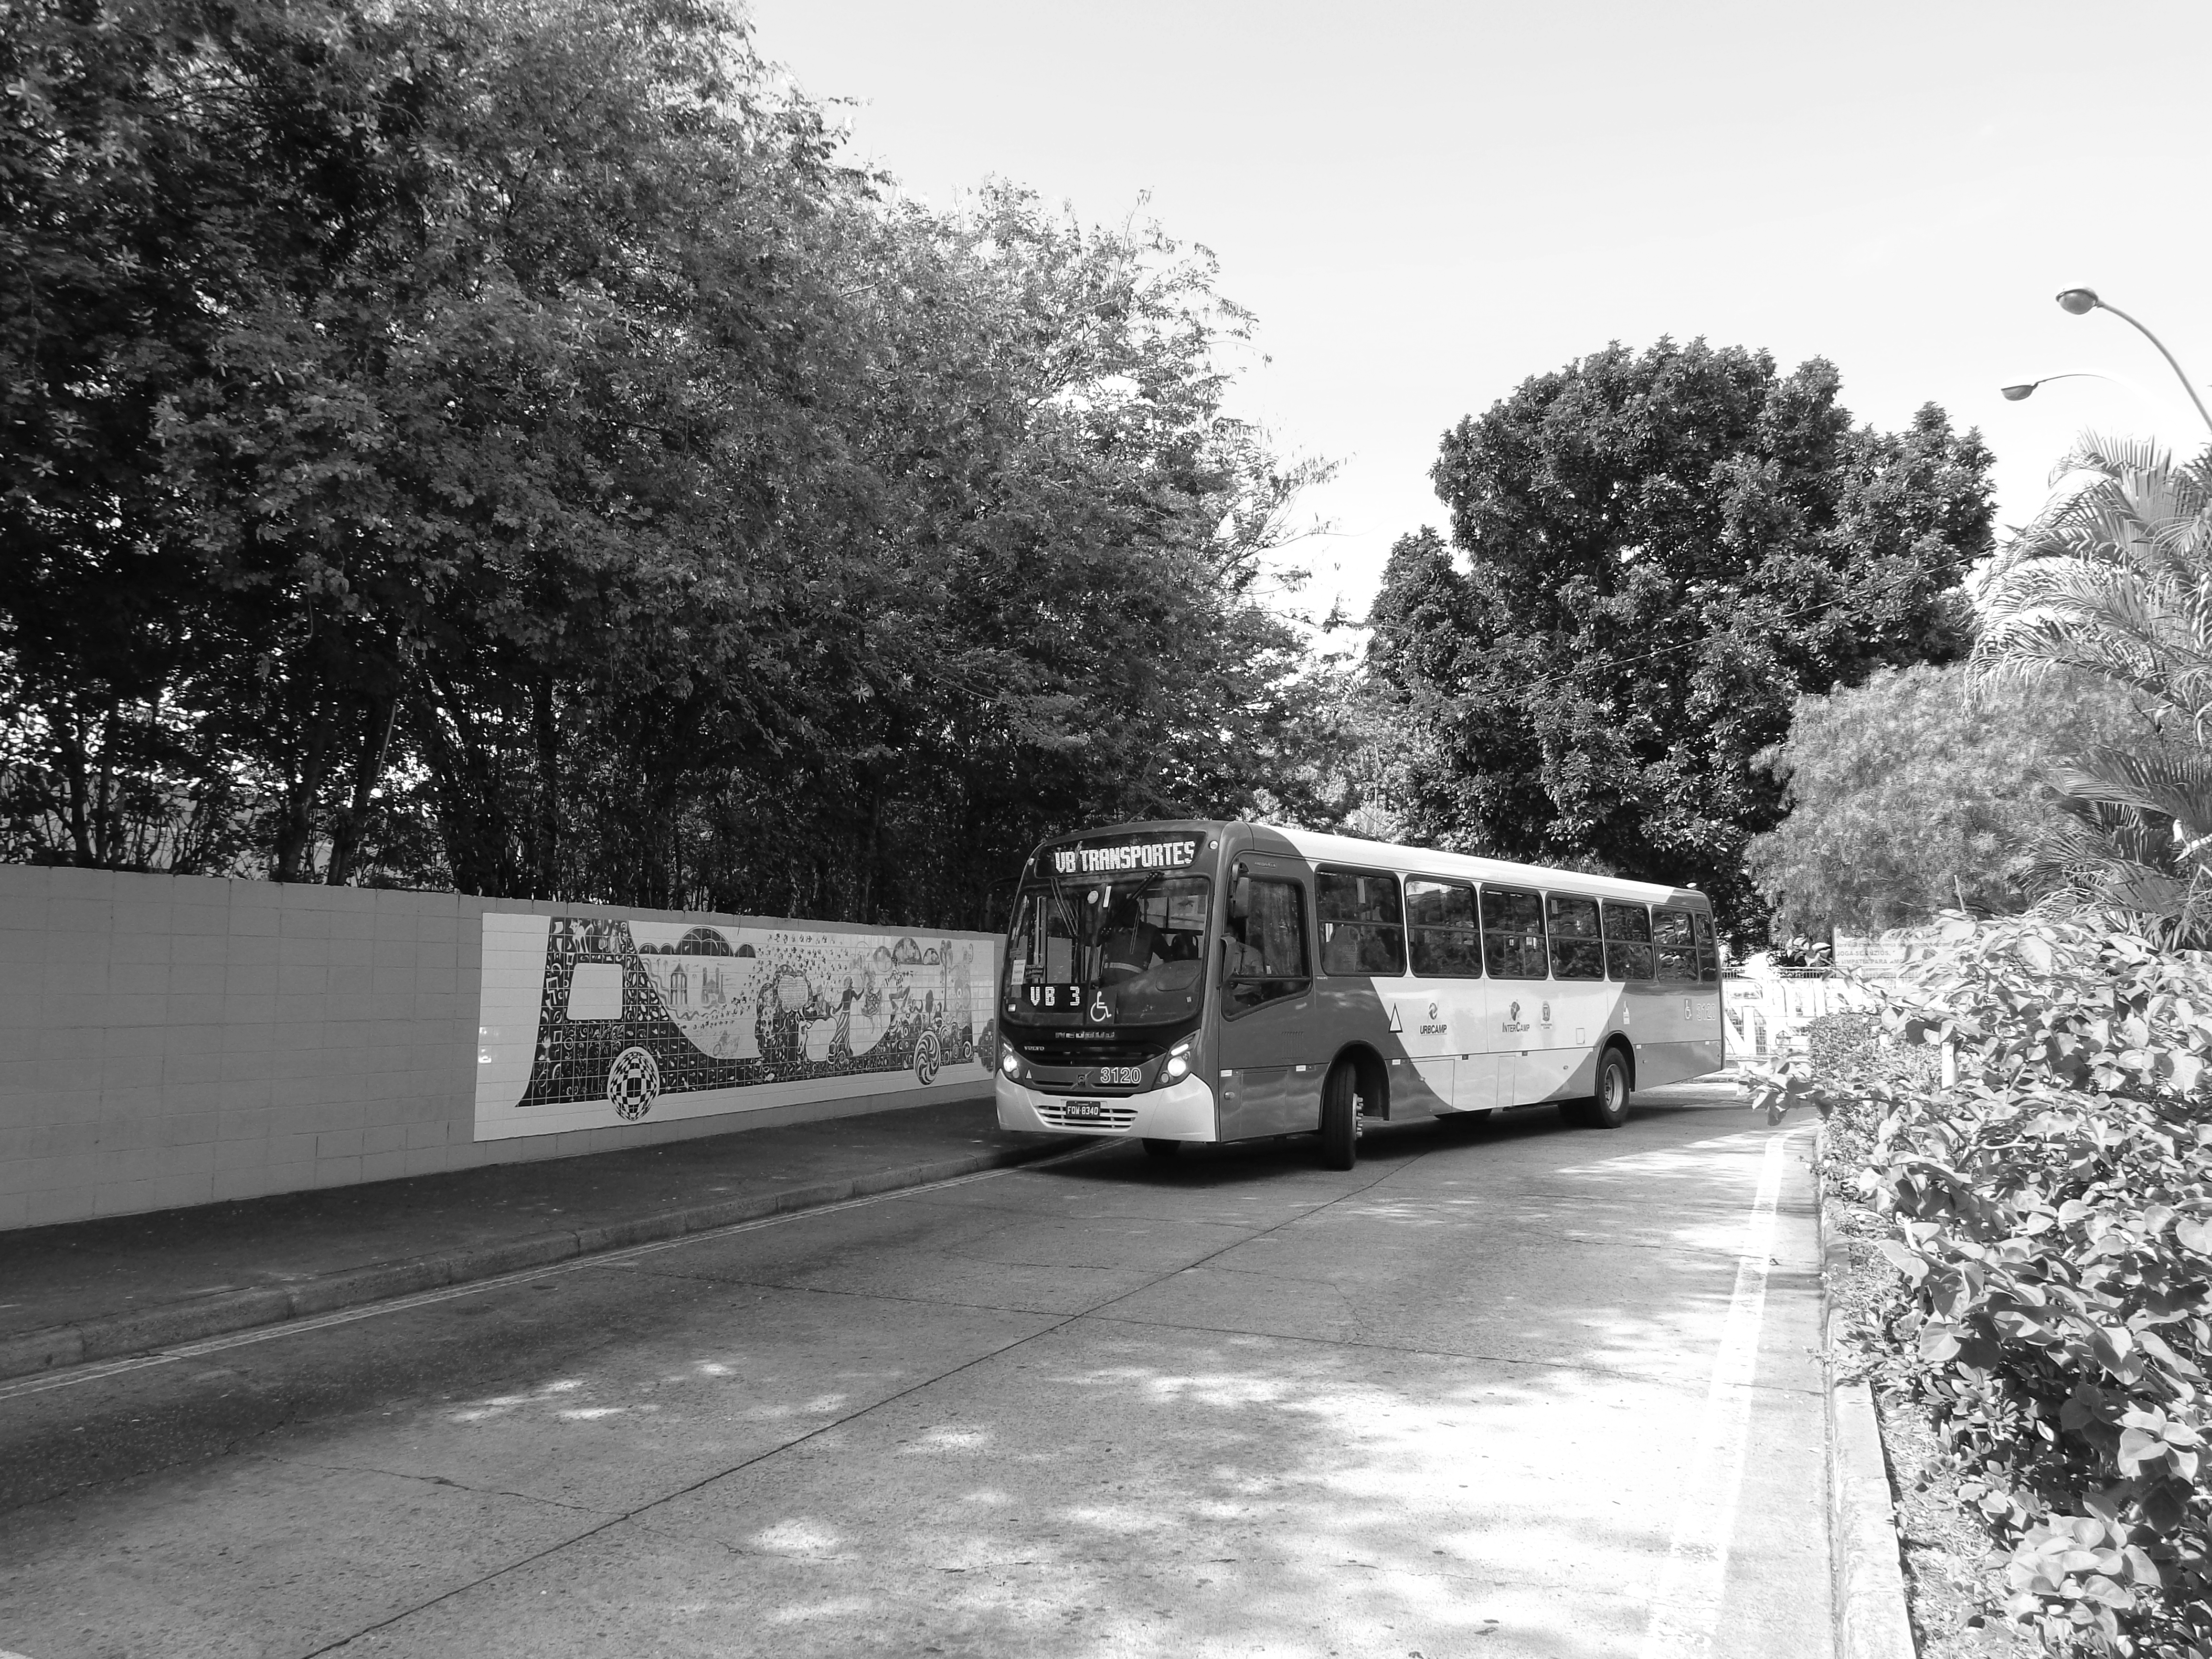
\includegraphics[width=.45\textwidth]{img/barao/onibus.jpg}
\end{figure}

O sistema de transporte público em Campinas é composto apenas por ônibus, e
chama-se InterCamp. O órgão municipal que organiza, gerencia e fiscaliza o
transporte público é a EMDEC (Empresa Municipal de Desenvolvimento de Campinas).
A bilhetagem eletrônica é organizada pela Transurc, a associação das empresas de
ônibus do transporte coletivo urbano de Campinas. Além das empresas, operam no
InterCamp cooperativas de transporte, originadas dos antigos perueiros.

Os ônibus em Campinas são identificados por um número de três dígitos, uma cor
(azul claro, azul escuro, vermelho ou verde), uma figura geométrica (círculo,
quadrado, triângulo ou tetragrama, para que os portadores de daltonismo possam
identificar os ônibus) e um nome.

A tarifa foi reajustada em janeiro de 2016 e custa R\$3,80 (quase dois bandecos)
.

Todo mês, em dois domingos, os usuários do transporte público de Campinas podem
usar os ônibus pagando metade da tarifa (o que dá R\$ 1,90). É o Passe Lazer. O
benefício vale apenas para passagens avulsas (sem cartão) e para o Bilhete
Único Comum.

Desde 2015, existe o Bilhete Único Universitário. Mais informações sobre ele
podem ser obtidas na seção sobre ele mais abaixo.

Existem quatorze linhas de ônibus que ligam o centro, alguns distritos, bairros e
terminais de Campinas ao distrito de Barão Geraldo. Algumas linhas desembarcam
os passageiros no terminal de Barão Geraldo, de onde seguem em outros ônibus
para a universidade. Já outras linhas vão direto para o campus. As trocas de
ônibus dentro do Terminal de Barão Geraldo são gratuitas, o que não ocorre em
outros terminais (no Terminal Mercado, por exemplo).

Em 2008 foi construída a nova e moderna rodoviária de Campinas, o terminal
multimodal Ramos de Azevedo. Além de transporte interestadual e municipal, o
espaço agrega um terminal metropolitano com o intuito de ligar as cidades da
Região Metropilitana de Campinas. Algumas linhas de ônibus internos de Campinas
também passam neste Terminal, como a linha 332.

Para consultar linhas de ônibus, há duas opções:
\begin{itemize}
  \item o sistema da EMDEC, que também possui um roteirizador bastante
interessante (\url{www.emdec.com.br/ABusInf/})
  \item o site Ônibus de Campinas, do Portal InterBuss, criado por entusiastas
de ônibus, dentre eles, um veterano da Computação
(\url{www.portalinterbuss.com.br/campinas/})
\end{itemize}

Outra ferramenta interessante para quem pretende usar o transporte público em
Campinas é o aplicativo Moovit, disponível para iOS, Android e Windows
Phone. Com ele, é possível visualizar os pontos de ônibus ao seu redor e as
linhas que passam neles. Além disso, também funciona como roteirizador,
indicando as linhas que você pode pegar para chegar a um lugar da cidade.

Para reclamações do transporte público, é necessário utilizar o canal 156 da
Prefeitura de Campinas. Ele pode ser acessado através do telefone 156, através
do site da Prefeitura (\url{www.campinas.sp.gov.br/servico-ao-cidadao/156.php}),
e através do aplicativo 156 Mobile Campinas, disponível para Android. As
reclamações são respondidas pelos órgãos de fiscalização da EMDEC, e todo o
processo pode levar até seis meses. Entretanto, é o único meio que pode resultar
em ações efetivas, como multas e advertências. Além disso, a reclamação entra
nas estatísticas da EMDEC, que são utilizadas para direcionar agentes de
fiscalização e, caso haja algum problema operacional de itinerário ou de
horário, também podem ser feitas alterações para otimização do serviço.

\subsubsection{Bilhete Único Comum}

O Bilhete Único foi implantado com o objetivo de facilitar o transporte daqueles
que se utilizam de ônibus. No prazo de 2 horas, o usuário pode usar até três
ônibus pagando apenas uma passagem. Além disso, agora o usuário tem dois
créditos negativos para utilizar caso o saldo seja zerado. O cadastro do
Bilhete Único Comum, em específico, é rápido e o cartão sai na hora.

O uso do Bilhete Único não é mais obrigatório, você pode pagar pela passagem
diretamente para o motorista. Entretanto, vale a pena fazer o cartão, mesmo
que você ande de ônibus muito raramente.


Os locais que fazem o Bilhete Único Comum podem ser consultados na página: 
\url{bit.ly/1Or5Tlm}.

Para a primeira recarga, exige-se o pagamento de uma tarifa (o que atualmente
fica em R\$ 3,80).

Para recarregar o cartão, além dos terminais, também tem diversos
estabelecimentos comerciais credenciados a fazer a recarga do cartão, que podem
ser vistos na página: \url{bit.ly/13Aav2C}.

\subsubsection{Bilhete Único Universitário}

Desde 2015, existe o Bilhete Único Universitário, voltado para estudantes que
necessitam do transporte público municipal para se deslocarem diariamente. Os
beneficiados pagam apenas metade da tarifa e possuem os mesmos benefícios de
integração dos usuários das demais modalidades do Bilhete Único.

Para obter o cartão, é necessário se cadastrar em uma área específica do site
da Transurc (\url{www.transurc.com.br/}), onde o estudante deverá preencher
um formulário, anexar uma foto e um comprovante de residência digitalizado.

Após enviar o formulário preenchido com os documentos anexados, a Transurc
irá avaliar se o pedido é procedente. O estudante pode acompanhar todo o
processo pelo site. Quando for aprovado, o sistema enviará um e-mail e deverá
ser pago um boleto com a taxa de emissão (equivalente ao valor de duas
tarifas comuns).

Após o pagamento do boleto, a Transurc deverá emitir o cartão em um prazo de
5 dias úteis. Quando estiver pronto, será enviado um e-mail e o estudante
poderá retirá-lo na sede da Transurc (Rua 11 de Agosto, 757).

O benefício só é concedido a estudantes que comprovem residência em Campinas,
que esteja a mais de um quilômetro da instituição de ensino, e que estudem em
uma instituição de ensino superior da cidade.

Outro detalhe importante é que o número limite de créditos possíveis para se
carregar mensalmente é proporcional à frequência do curso informada pela
universidade. Alunos da EC e da CC podem carregar 50 créditos mensais, pois
a Unicamp informou à Transurc frequência de 5 e 6 dias semanais,
respectivamente, independente do número de créditos em andamento de cada
pessoa.

A recarga do Bilhete Único Universitário pode ser feita nos postos da
Transurc e em qualquer estabelecimento da rede credenciada
(\url{bit.ly/13Aav2C}).

